\documentclass{witrman}
\usepackage{wrapfig}

\title{DJ TRAINING MANUAL}
\date{SPRING 2019}
\renewcommand{\TitlepageGraphic}{images/titlepage}

\begin{document}

\maketitle

\maketoc{}

\setpagebg{}

% Friendly reminder: use \textbf{} for emphasis.
% Underlines are typographically ugly!

\chapter{Becoming a DJ at WITR}

DJs are the face of WITR's whole operation, and are the gatekeepers of our
on-air broadcasts.  WITR's weekly show schedule consists of live DJing from
students and community members, who all bring their own diverse tastes in music
and styles to the table.  DJing allows members to discover new music, improve
communication skils, and represent WITR as an organization.  Running the board
is truly a lot of fun, but keep in mind that it also requires preparation and
passion.  This manual will help you to prepare for the responsibilities that a
% This \@ means that you want LaTeX to use "intersentence spacing."  In
% non-typographer terms, it's a hint that you want the larger spacing to be
% after the period, rather than before it.  Generally, you use this when you end
% a sentence with an abbreviation or capital letter.
DJ has at WITR\@.

The process to become a DJ at WITR consists of several steps, through which your
trainer will guide you:

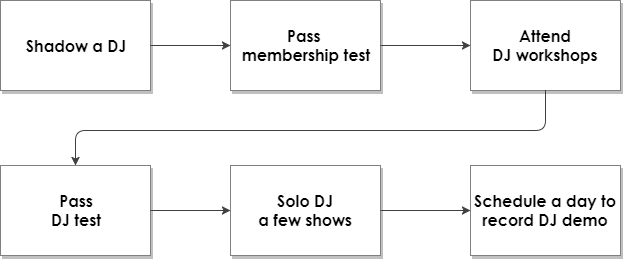
\includegraphics[width=\textwidth]{images/dj-flow.png}

Shadowing a DJ is meant to introduce you to some of our DJs and to let you
decide whether or not you want to become a DJ at WITR yourself.  After
shadowing, if you have decided that DJing is something you want to pursue, you
must first pass the All Member Test before you can begin training.  DJing is a
privilege, reserved strictly for members of the station.  Once you are
officially a member, the Program Director will pair you with one of our seasoned
DJ trainers.  Your trainer will work with you for one hour sessions once a week
to develop your skills and get you into the groove of DJing.

When they feel you are ready, your trainer will arrange for you to take our
written DJ test.  Everything that will be on the test can be found in this
manual, although you will likely find that after working with your trainer for
several weeks, you will know most of the information already.

Upon passing this test, you will DJ for several one hour, supervised shows to
demonstrate that DJing has become second nature to you.  You can then schedule a
time and day with your trainer to record a two hour DJ demo.  Your trainer will
supervise the Underground feed from the station office, but you will DJ alone in
the studio for these hours.  The Program Director will then review your demo and
grade your performance based on a rubric derived from this training manual,
which takes into account your timing, style, transitions, and more.

After passing your demo, you will officially be authorized to DJ on air in
Studio X\@!

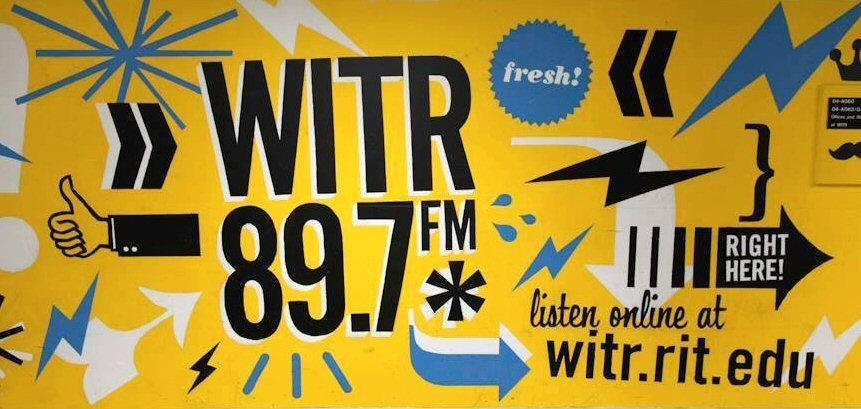
\includegraphics[width=\textwidth]{images/witrwall.jpg}

\chapter{Programming}

We are a proudly versatile station in terms of programming.  While WITR 89.7 is
primarily an indie-based station, we also broadcast a variety of genre-specific
specialty shows in addition to shows that feature local artists, artist
interview pieces, sports commentary, and weekly news.  As a DJ, you will have
many opportunities to discover new music and make your Pulse of Music show
unique to you.  No two DJs are quite the same in their musical style choices,
and our listeners get to experience a diverse range of genres as a result.

WITR is not a completely free-form station when it comes to content.  There are
developed rules and guidelines in place to ensure that our DJs and our audience
can enjoy professional, high-quality broadcasting.  It is vital that you adhere
to the following format and are knowledgeble of WITR's on-air requirements when
you're operating the studio.

\subsection{The Pulse of Music Format}

The Pulse of Music is a mainstay of WITR's daytime and weekday programming.
Every DJ is trained first and foremost in the Pulse of Music format and by
default, when no DJs are on the air, our automation system plays Pulse of Music
content.  This format is what we have determined to be the best balance between
new and interesting content for our listeners, and great creative freedom for
our DJs.  The end result is a professional, catchy broadcast style that
represents the station's tastes as a whole.

A Pulse of Music show is typically 2 hours long, but can be broken up into two
separate 1-hour long shows if necessary.  Pulse of Music shows may only play
music owned by WITR\@.  DJs can select their onw music from our vast library
downstairs, our bin of new albums, and our racks of local music.  This by no
means limits our DJs' options, as our library consists of thousands of CDs from
every genre --- and the second largest private vinyl collection in
New York State.

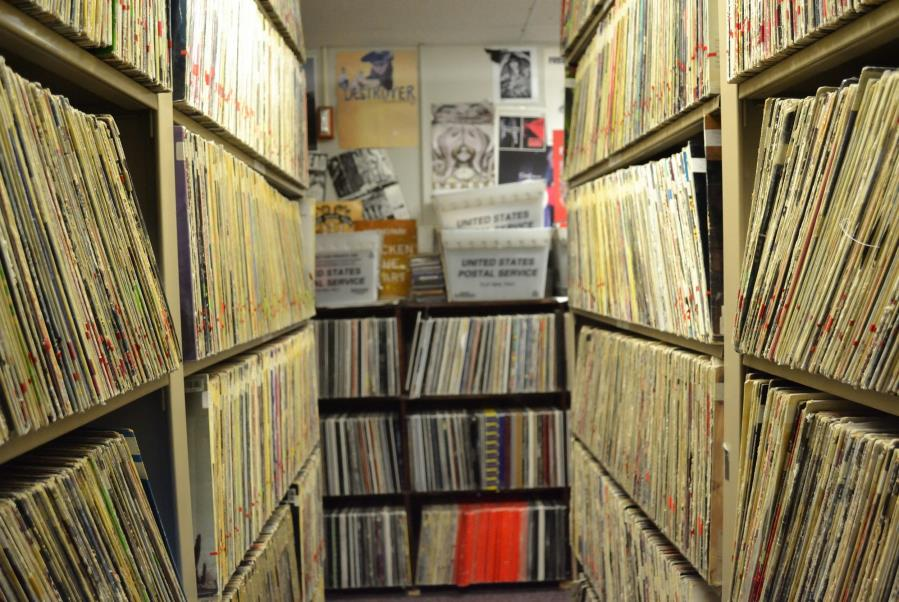
\includegraphics[width=\textwidth]{images/library-vinyl.jpg}

\subsection{Components}

There are several different types of content that a Pulse of Music show may
contain.
\begin{itemize}
    \bolditem{New Bin}{Our new music from the past 3 months.  Albums are
        regularly cycled in and out of the New Bin.}
    \bolditem{Feature}{Particularly awesome tracks that we really want to expose
        our audience to.  Features are decided at open meetings once a week.
        Any member is welcome to attend and contribute their opinions.}
    \bolditem{Recurrent}{This is where feature tracks are moved after they're
        done being featured.  The entire album a feature was on is considered
        recurrent, not just the featured track.}
    \bolditem{Specialty}{Several racks of albums frequently used for specialty
        shows}
    \bolditem{Double Shot}{A ``double shot'' is when you play two songs
        by the same artsit consecutively.  The tracks \textbf{must} be played
        back-to-back, but do not need to be from the same album.}
\end{itemize}

% This creates a table with two columns, each one centering its contents.
% The border between two columns is an ampersand (&), and the end of a row is
% indicated by two backslashes (\\).  Note that no rules are drawn around these
% table cells. Between-column rules are specified in the second pair of curly
% braces with a pipe character (|).  Between-row rules are drawn with \hline
% after the row-end marker.
\begin{tabular}{cc}
    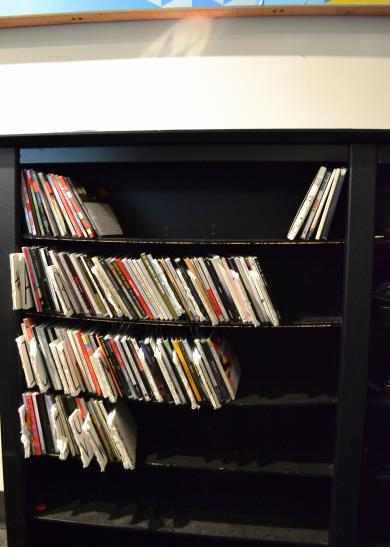
\includegraphics[width=0.47\textwidth]{images/newbin.jpg} &
    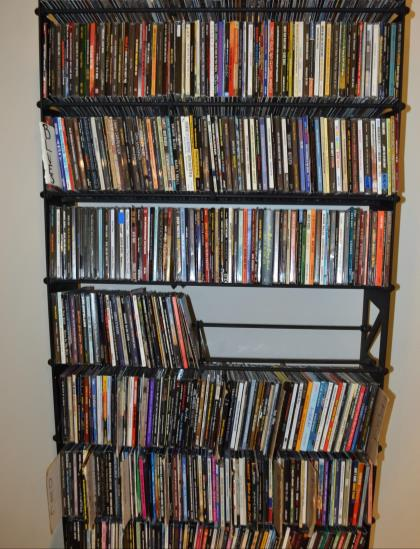
\includegraphics[width=0.47\textwidth]{images/specialty.jpg} \\

    New Bin &
    Specialty Show Rack \\
\end{tabular}


\subsection{Structure}

A Pulse of Music show \textbf{must} contain these elements:

\begin{tightitemize}
    \item New Bin: at least 50\% of the music you play
    \item Features: 2 per hour
    \item Recurrent: 1 per hour
\end{tightitemize}

Except for double shots, the same artist \textbf{should not} be played more than
once every 2 hours.

A double shot can only be played once per hour.  You can also play up to two
specialty show tracks an hour, provided that you follow up these tracks by
mentioning the specialty show they are from, and the day and time that show
occurs.

\subsection{Imaging}

As you'll know from listening to radio yourself, a broadcast does not consist
solely of music.  The songs are punctuated by various advertising, promotions,
and sound bites, and WITR is no different.  Any audio clip that isn't a song is
called ``imaging.''

Our imaging at WITR is made of audio files that have been cut and edited by our
production department.  These sound clips are incredibly important for the
station's image, for our business department, and for FCC compliance.  Playing
WITR-specific promos lets our listeners know what station they're tuned to and
conveys our station's personality in between sets.  Underwriting spots can be
sold to local businesses and RIT clubs to generate revenue for the station.
Additionally, the FCC requires us to play certain imaging by law.  Ultimately,
WITR uses several different types of imaging:

\begin{itemize}
        \bolditem{Legal ID}{Our call letters immediately followed by the
        community we serve.  For us, this is ``W-I-T-R Henrietta.'' You must
        pronounce the individual letters of WITR\@; ``witter'' is only a
        nickname.  A legal ID must be played \textbf{once an hour, at the top of
        every hour, give or take 5 minutes}.  The legal ID may also be spoken
        during a mic break, preferably the first natural mic break near the top
        of the hour.}
        \bolditem{PSA}{A ``Public Service Announcement'' written by the
        National Ad Council.  These are provided to us by the Ad Council and
        come in three different lengths, 15, 30, and 60 seconds.  A PSA (of any
        length) must be played \textbf{once an hour}.}
        \bolditem{Specialty Show Promo}{A promotional clip highlighting any one
        of WITR's weekly specialty shows.  You must play \textbf{one promo per
        hour}.}
        \bolditem{Underwriting}{This is a way for WITR to acknowledge donations
        from businesses without making any ``calls to action.''  Underwriting is
        scheduled for \textbf{specific time slots on certain days} and must be
        played at these times, which will be noted in the weekly logs.}
        \bolditem{Weekend Events}{A summary of upcoming RIT events, usually
        voiced by our own station members and edited by the News Director.  Like
        underwriting, we don't always have a weekend event imaging recorded.
        When we do, they must be played \textbf{once every 2 hours}.}
        \bolditem{Shotgun}{A 2--5 second sound bite that includes ``WITR 89.7''
        or just ``WITR.''  These promote our station and create natural
        transitions between songs.}
        \bolditem{Sweeper}{A 10--30 second sound bite that gives information
        about WITR\@.  There are two types of sweepers: attitude and position.
        Position sweepers reflect the station and its contributions to the
        public.  Attitude sweepers tend to be more tongue-in-cheek.}
\end{itemize}

The last two imaging types listed are self-promotional; they boost WITR's image
and convey our station's character. DJs can choose which promotional spots to
play at their own discretion, but listeners should hear ``WITR'' roughly
\textbf{once every 8 minutes}.


\subsection{Specialty Show Format}

The format of a Specialty Show is vastly different from that of a Pulse of Music
show.  Specialty Show DJs can play from a certain artist any number of times,
aren't required to include New Bin content, and only have to play legally
required imaging (PSAs and Legal IDs).  Specialty Shows are specific to a single
genre or theme, and because of this narrowing of music choices, DJs are allowed
to bring their own music to play on air.  Additionally, Specialty Show DJs often
elaborate a great deal on the music they play, which results longer, more
in-depth mic breaks.  Specialty Shows have their own names, imaging promos, and
featured banners on the WITR website.  A few examples of Specialty Shows include
reggae, blues, disco, world, jazz, electronic, punk, metal, and many more.

\begin{tabular}{*{4}{m{0.23\textwidth}}}
    
\includegraphics[height=0.23\textwidth]{images/reggae.jpg} &
    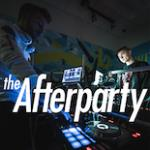
\includegraphics[height=0.23\textwidth]{images/afterparty.jpg} &
    
\includegraphics[height=0.23\textwidth]{images/13thfloor.jpg} &
    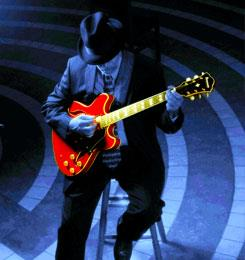
\includegraphics[height=0.23\textwidth]{images/blues.jpg} \\

    % \footnotesize selects a smaller font
    % \centering turns on centering
    % Both of those macros affect the current scope, which in this case is the
    % table cell.  That's why they're duplicated for each cell.
    \footnotesize \centering Reggae Sounds with Babi Katt &
    \footnotesize \centering The Afterparty with Fluent and Stoph &
    \footnotesize \centering 13\textsuperscript{th} Floor with Johnny Thunder &
    \footnotesize \centering Bad Dog Blues with Gary \\
\end{tabular}


\chapter{On-Air Rules and Regulations}

In addition to the general station policies and FCC regulations, DJs must adhere
to certain protocols while operating in the studio.  It is crucial that you know
these procedures by heart, as failure to comply with the following rules can
result in suspension or expulsion.

\subsection{Before Each Show}
\begin{tightenumerate}
    \item Sign in on the daily FCC log.
    \item Take a power reading and record it in the FCC log.
    \item Review the imaging log to ensure you know which sound bites to play in
        a given week.
\end{tightenumerate}

Don't forget to be respectful of the DJ in the studio before you.  Wait outside
the studio until they have left, and if they are still playing at the time of
your slot's start, politely remind them that it is your hour to DJ\@.  If they
refuse to yield the studio, contact the Program Director.  It is recommended,
that you use any pre-show time to plan a few sets.

\subsection{After Each Show}
\begin{enumerate}
    \item Announce the next upcoming DJ or show during your last mic break.
    \item Sign off in the daily FCC log.
    \item Make sure that either the next DJ has taken control of the studio, or
        that you have turned on automation and noted this in the FCC logs.
    \item Restore the board settings, studio lights, and studio setup to how you
        found them.
        % Restore the board settings, studio lights, and studio setup using WITR
        % Standard PRocedure (WSPR) № N
    \item Clean up all CDs, records, and other materials that you may have used
        during your show.  Return them to their proper location in the library.
\end{enumerate}

\subsection{Missing a Show}

It's understandable if you have to miss a show every now and then, but remember
there is a responsibility that comes with having a weekly show.

If you cannot make your time slot, you must do the following:

\begin{enumerate}
    \item Notify the Program Director as soon as possible.
    \item Let the DJ before you know that you won't be there to take over after
        thier show.
    \item Find a substitute DJ to run your show in your place.  Most DJs do
        this by either posting on Facebook or putting a sign up in the office.
    \item If you can't find a substitute and your show is at least 1 day away,
        voice track the show in Studio B.
\end{enumerate}

Having a regular show is a privilege.  Depending on scheduling each semester, it
is not unusual for two DJs to want the same time slot.  If you were awarded this
spot, but often miss your show, you are depriving a fellow DJ of a show that
they would love to run.

If your show time begins to pose a conflict for you, inform the Program Director
and request to move your show.  Missing 3 shows without prior approval of the
Program Director will result in a \textbf{loss of on-air privileges}.


\subsection{Suspensions}

Suspendable offenses include:

\begin{itemize}
    \item Improper sign-off/sign-on.  Do not leave the station without
        automation running.
    \item Not properly keeping the daily FCC logs.
    \item Broadcasting obscenity, profanity, or indecency (including during a
        mic break or musical content).
    \item Playing music that isn't from the WITR library during a Pulse of Music
        show.
    \item Failing to play at least 50\% New Bin on a Pulse of Music show
    \item Missing 3 shows without prior excuse from the Program Director
    \item Behaving inappropriately in the station (including the studios, the
        office, the garage, and the pit).
    \item Not maintaining volume levels (either too loud or too quiet).
    \item Breaking any other programming rules as laid out by station policies
        and the Program Director
\end{itemize}

If you notice another DJ in violation of these rules, you are required to notify
the Program Director immediately.

Suspensions are issued at the discretion of the Program Director, Chief
Engineer, and General Manager.  Any one of these E-board members is capable of
suspending your on-air privileges.  The duration of a suspension depends on the
severity of the offense, and is also at the discretion of the E-board.

Try to never be on the receiving end of one of these:

\begin{center}
    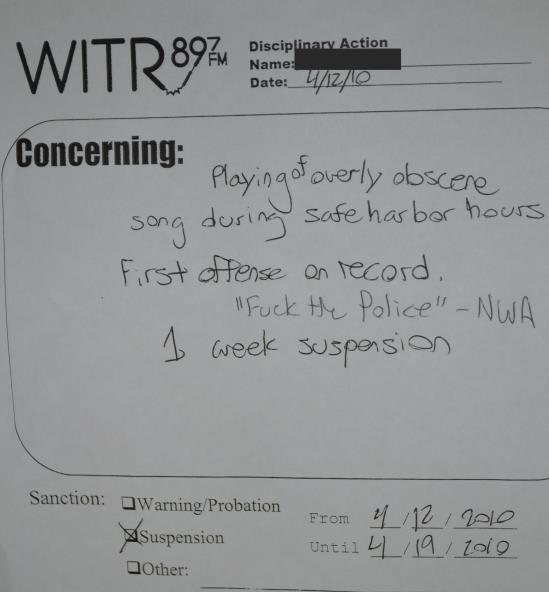
\includegraphics[height=0.4\textheight]{images/fthepolice.jpg}
\end{center}

No E-board member \textbf{wants} to give out suspensions, and will automatically
give a DJ the benefit of the doubt.  Everyone at WITR wants to see the station
function seamlessly and for DJs to continue rocking the studio at their freedom.
E-board members will always wait to assign a suspension until they have
confirmed firsthand that an offense transpired.


\chapter{Studio Equipment}

In both Studio A and Studio X, there is a myriad of equipment that enables us to
broadcast.  It is a DJ's job to know how each of these pieces of equipment works
and to regularly operate the studio as a whole.

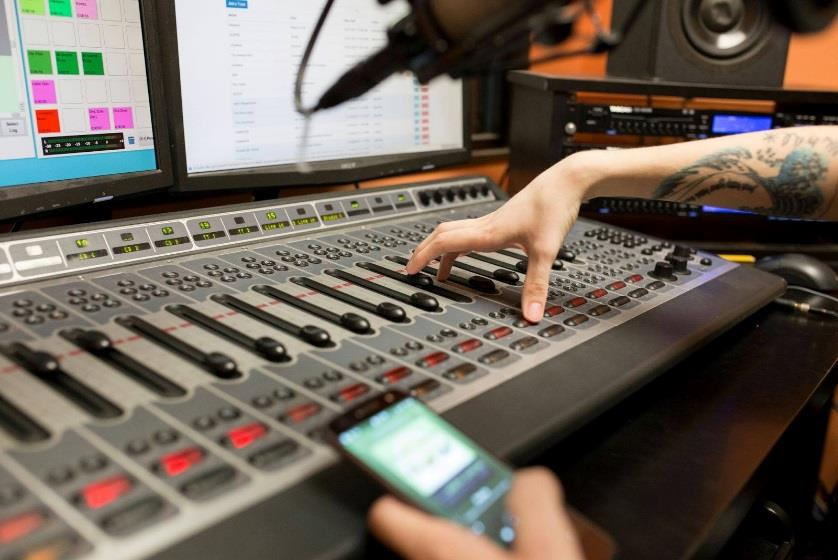
\includegraphics[width=\textwidth]{images/console.jpg}

Easily the most important piece of equipment the DJs use is the Studio Console,
also colloquially referred to as ``the board.''  Everything that you will
broadcast during a show goes through the board, which consists of many different
parts you will need to understand.  Don't let this intimidate you, though!
Working the board will become second nature to you throughout the course of your
training.

{\centering 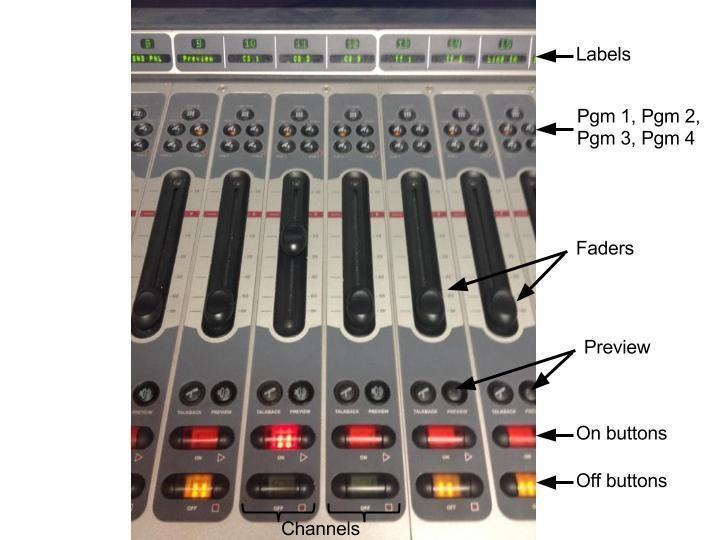
\includegraphics[width=0.75\textwidth]{images/faders.jpg} }

\subsection{Channels}

The 20 thin, vertical stripes (panels) on the board control different channels,
each of which has a different input source, indicated by the small screen at the
top of the panel.  Channels have a red ``On'' button which sends the channel's
output over the air.  This also initiates playback of a source, meaning that if
you have a CD or vinyl cued up, turning on the channel will begin playing that
CD or vinyl.  Note that pressing the ``On'' button again will not start playing
the source if the channel is already on.

Each panel also has an orange ``Off'' button, which mutes all output from a
channel.  As long as a channel is turned off, no audio will go out over that
channel, regardless of where the fader is.  However, it is poor practice to
leave a channel on when you are not using it, as this leaves you open to
accidentally sending audio out over the air.  After using the \textbf{mic, CD,
vinyl, or line channels}, be sure to \textbf{turn them off}.


\subsection{Assignment Switches}

Above and below each channel's fader is a group of small, circular buttons,
referred to as Assignment Switches.  Each switch has a different function:

\begin{tightitemize}
    \bolditem{PGM 1}{Sends to the transmitter}
    \bolditem{PGM 2}{Sometimes used to preview audio}
    \bolditem{PGM 3}{Used to test equipment}
    \bolditem{PGM 4}{Patches through the VoxPro call recorder as well as the
    Access remote unit}
\end{tightitemize}

Ask the Chief Engineer for more information about equipment testing and VoxPro
operation.

\begin{itemize}
    \bolditem{Preview}{Turns down the volume of the monitors and pushes a
        channel's audio directly to the headphones.  Press the ``Preview''
        button to listen to a channel before sending it over the air.  To be
        safe, always make sure this channel's fader is down so you don't
        accidentally broadcast the audio.  Also, don't forget to \textbf{turn
        Preview off before attempting to broadcast} from the channel.}

    \bolditem{Talk Back}{Allows the DJ to talk to the guest studio without also
        talking on air.  This feature \textbf{should not be used while the mic
        is on}, as it won't mute the mic.  While a guest's mic is off, hold down
        the ``Talk Back'' button on their channel to speak directly to them.}

    \bolditem{Headphones Knob}{Controls the volume of your headphones.}

    \bolditem{Monitor Knob}{Controls the volume of the studio's speakers.}
\end{itemize}

\subsection{Microphones}

\begin{itemize}
    \bolditem{Studio A Control Room Mic}{This microphone is operated only by the
        DJ running the board, and is in a separate room from the guest mics.
        When the mic is turned on, a light in the hallway also turns on to
        notify other people that you're live on air.}

    \bolditem{Studio A Guest Mics}{These are microphones set aside specifically
        for guest usage.  The DJ in Studio A is in charge of the guest mic
        levels and can turn them on and off.  The guests do not have volume
        faders on their side, only on/off buttons.}

        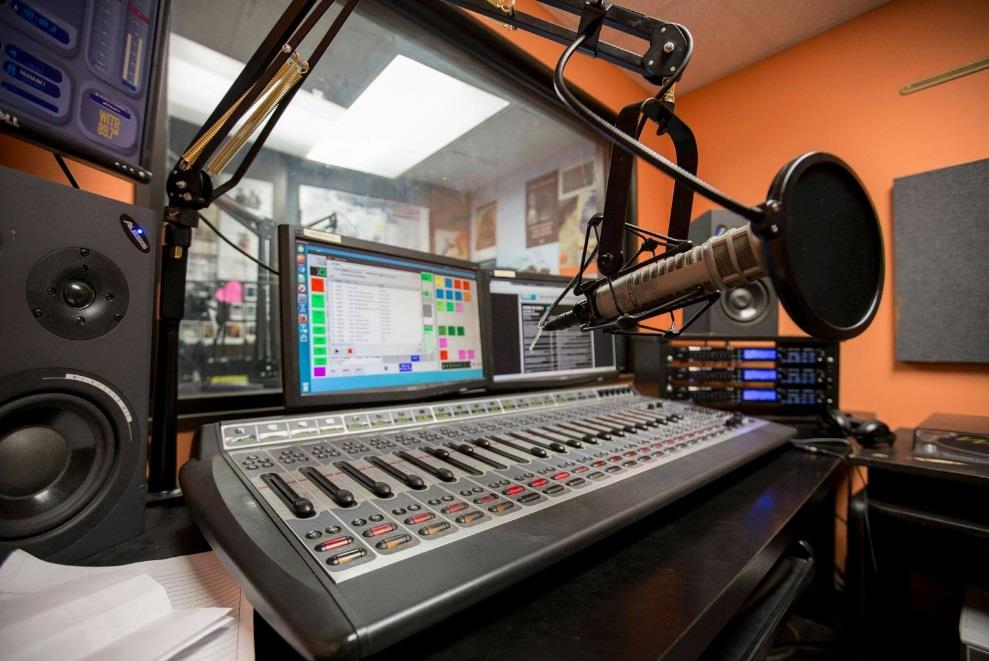
\includegraphics[width=\textwidth]{images/studioa.jpg}
        % TODO: Fix centering here

    \bolditem{Studio X DJ Mic}{The DJ mic in Studio X is in the same room as the
        guest mics, which renders the ``Talk Back'' button largely useless.
        When any mic is turned on, a ring around the mic will glow red.  Note
        that there is no on-air light in Studio X, so make sure you close the
        door before going on-air.}

    \bolditem{Studio X Guest Mics}{Like the DJ mic, each of the Studio X guest
        mics have a ring light to indicate whether they are turned on.  Unlike
        in Studio A, the guests have no control over their mics.}

        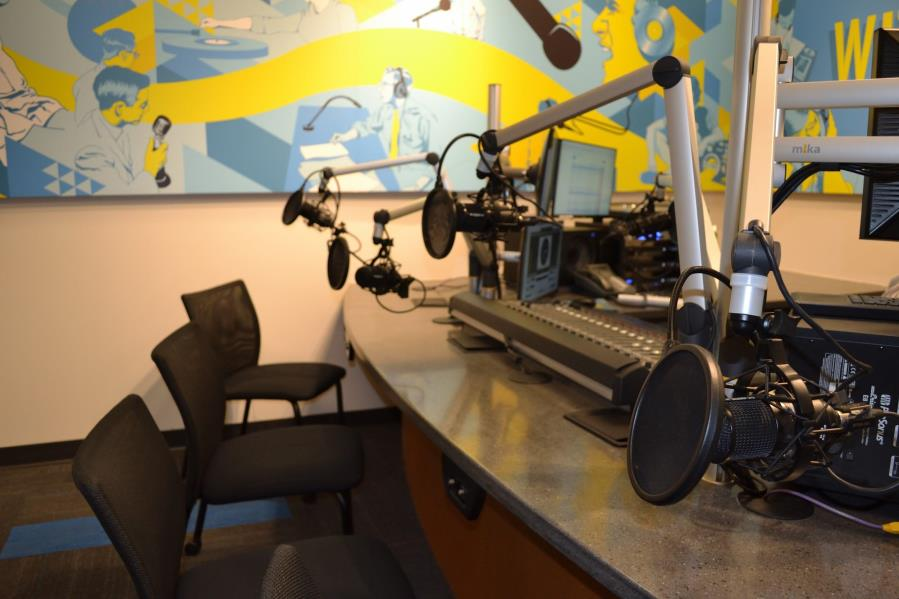
\includegraphics[width=\textwidth]{images/studiox.jpg}
        % TODO: Fix centering here
\end{itemize}


\subsection{CD Players}

In each of the studios, there are 3 CD players stacked up which, in order from
top to bottom, are controlled by the channels ``CD1,'' ``CD2,'' and ``CD3.''
After selecting a track, do not press play on the CD player.  Turning on the
channel will do this for you.  When you want to eject a CD, \textbf{press the
``Stop'' button before the ``Eject'' button}.  The CD players will not eject a
CD that is not stopped.  If a CD player stops working (or eats a CD), submit an
Equipment Support Ticket through the online DJ portal (covered later).

The CD players do have subtle operational differences between Studios A and X.
In Studio A, you can skip to a track by pressing the ``Skip'' button, and the
play time count begins at 0.  In Studio X, you can skip to a track by using the
``Tune'' knob, and the play time count begins at the song's duration and counts
down.

\begin{tabular}{cc}
    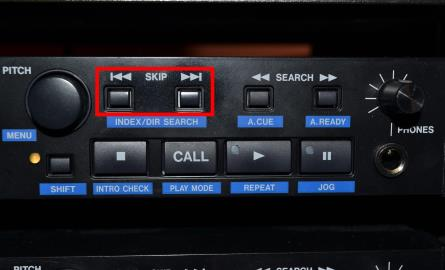
\includegraphics[width=0.46\textwidth]{images/cdskip.jpg} &
    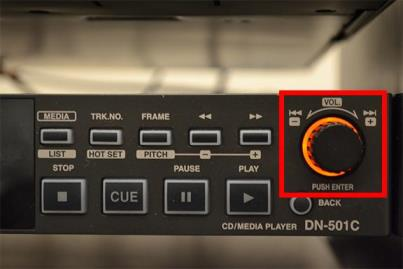
\includegraphics[width=0.46\textwidth]{images/cdvol.jpg} \\

    Studio A &
    Studio X \\
\end{tabular}

% TODO: add captions

A piece of advice that has been passed down by DJs through the ages: place a
CD's case on top of the player it's in.  That way, you know which case to put it
in when you're done, and you can more easily back-announce the tracks you played.

\subsection{Turntables}

There are two turntables in each studio which DJs use to spin vinyl records.
They are controlled by the channels labeled ``TT1'' and ``TT2.''

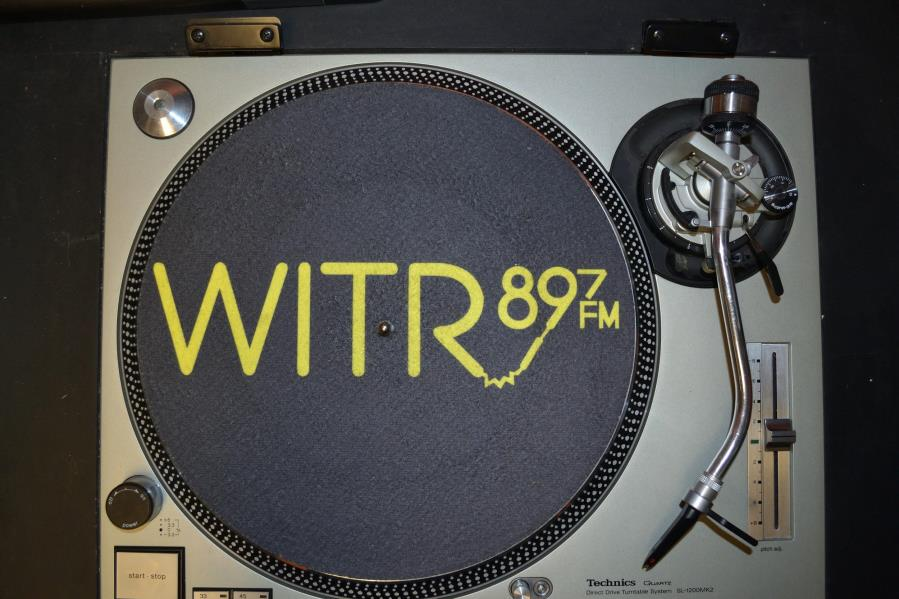
\includegraphics[width=\textwidth]{images/turntable.jpg}
\pagebreak

To prepare a track to play on air:
\begin{enumerate}
    \item Switch the turntable on (knob on the lower-left corner) and set it to
        either 33 or 45 RPM, as appropriate for the record.
    \item Put the turntable's channel on preview and \textbf{carefully} drop the
        needle using the cueing level.  Press ``Start'' to play the vinyl and
        stop the record once you hear sound.
    \item Rotate the platter (the disc where the vinyl rests) counterclockwise
        about 180º.  This gives the record time to speed up, and avoids a pitch
        shift at the start of the record.
    \item Turn on the corresponding ``TT'' channel and make sure it is potted
        up.
    \item Manually press ``Start'' on the turntable to play the track.
\end{enumerate}

\subsection{Dump Button}

This is the DJ's trusty ``Oh s---!'' button.  All shows, with the exception of
live hockey broadcasts, must run on a 5 second delay.  This is to prevent
FCC-inappropriate material from being broadcast over the air.  If you
accidentally speak or play an FCC-violating sound bite, hitting the dump button
catches the broadcast up to real-time, effectively preventing the last 5 seconds
of audio from playing.  (Unfortunately, this doesn't alter the online stream.)
The broadcast will then gradually slow down to achieve a 5 second delay time
again.  This means that the dump button cannot be pressed repeatedly in a short
time to skip more than 5 seconds of audio.

\subsection{Levels}

The soundboard's faders control the levels of the audio being sent over the air.
The computer monitor displays these levels as they occur during a broadcast.

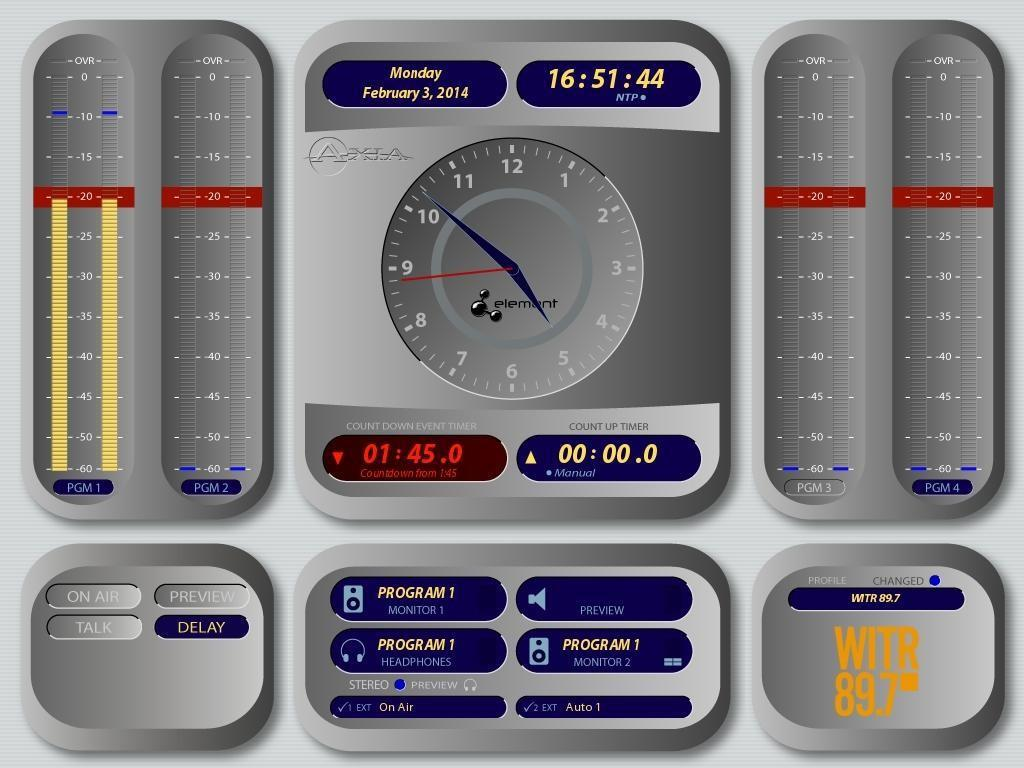
\includegraphics[width=\textwidth]{images/elementstatus.jpg}

The red lines mark the maximum volume our broadcasts should have.  Not only is
there a legal limit to our broadcast levels, but our audio quality begins to
degrade quickly above the red line.

The level meters are also a good indicator of whether or not you are speaking
too quietly during a mic break, a common problem for DJs. Always keep an eye on
your levels throughout a show, and adjust the faders accordingly.  Try to keep
levels consistent during your show, focusing on transitions between mic breaks
and music.

\subsection{Song Logger}

Every song that goes over the air must be logged in our online song logger.
This is required by the FCC and will be looked at every time the Program
Director does airchecks.  The logger can be found at
\href{https://logger.witr.rit.edu}{logger.witr.rit.edu/}, and it is encouraged
that you include this link in your mic breaks for any listeners who want to know
``what was that song you just played?''  The most recent song entered into the
logger will be displalyed on WITR's website under the ``Now Playing'' banner.

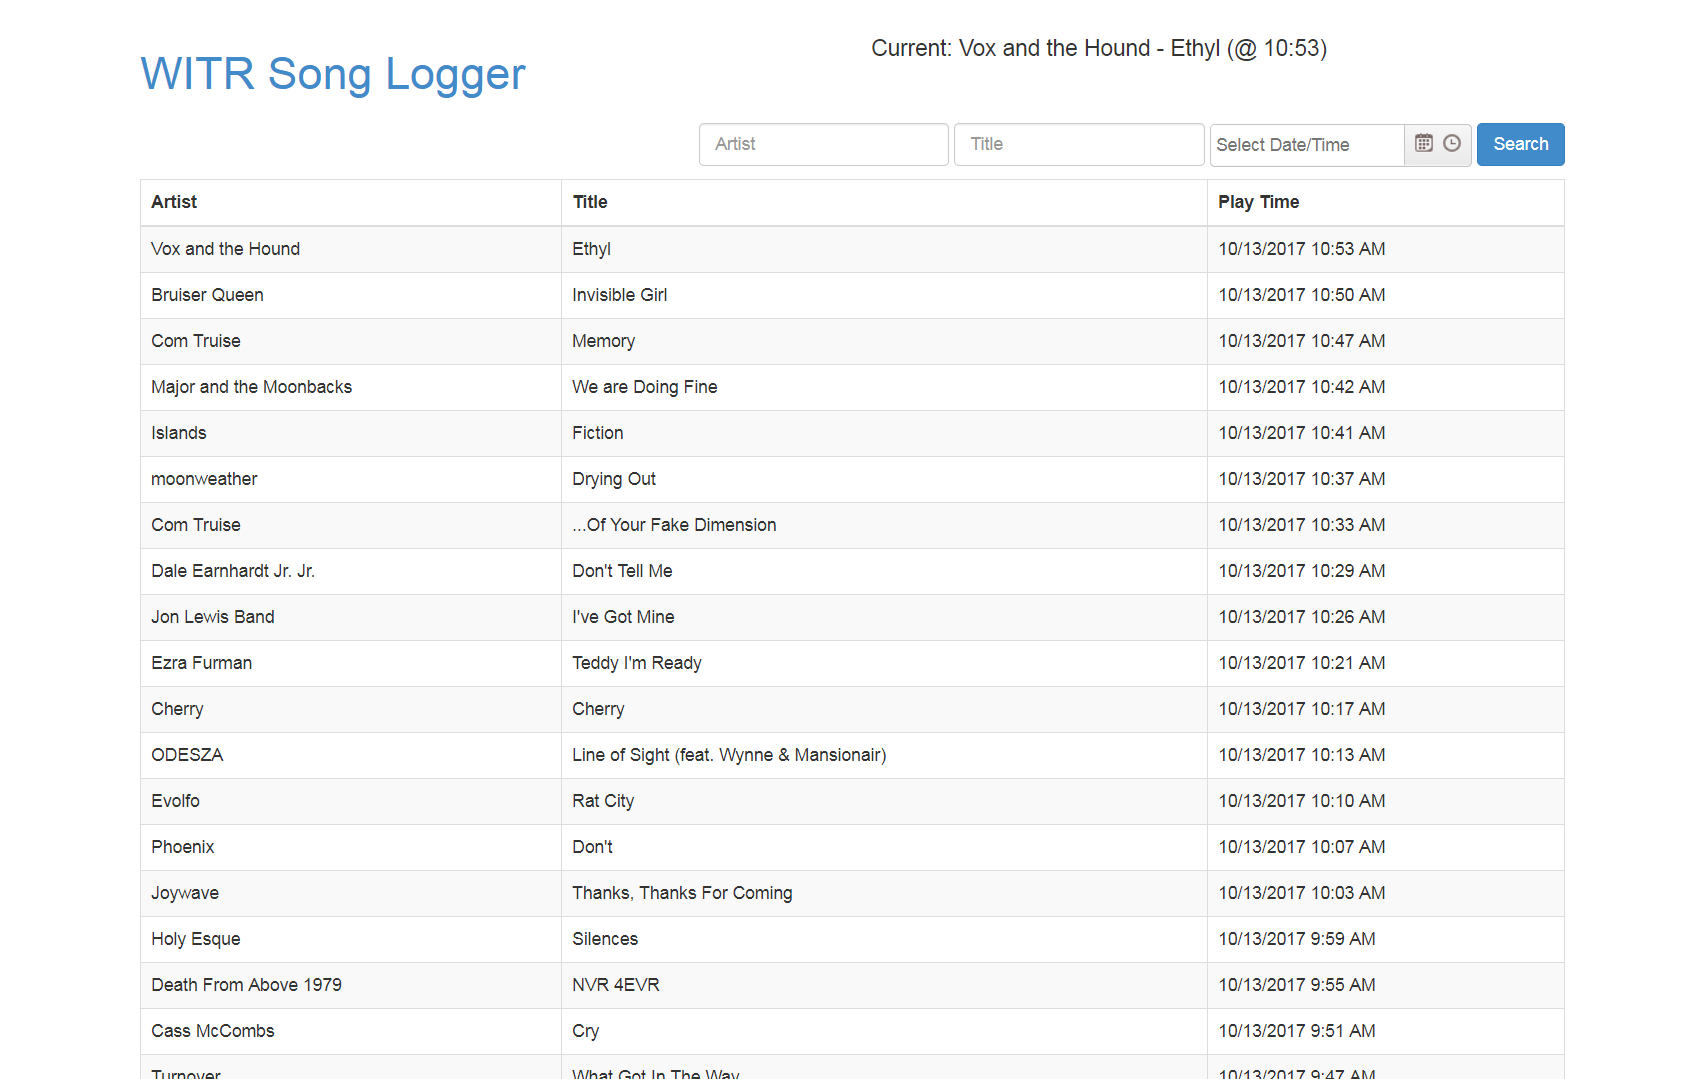
\includegraphics[width=\textwidth]{images/logger.png}

When logging music, you must include the artist name, song title, time played,
and section (new bin, library, request, etc.) in the logger entry as shown
below.  Try to be as accurate as possible with spelling and time played, because
all of our logs are public.  You won't have to manually log all of your songs,
since tracks played through Rivendell are automatically logged for you.  In the
event that the online logger is not working, you must write down your sets on
paper and submit the paper to the Program Director after your show.  Also,
immediately inform the Chief Engineer
(\href{mailto:engineer@witr.rit.edu}{engineer@witr.rit.edu}) that the logger is
down.

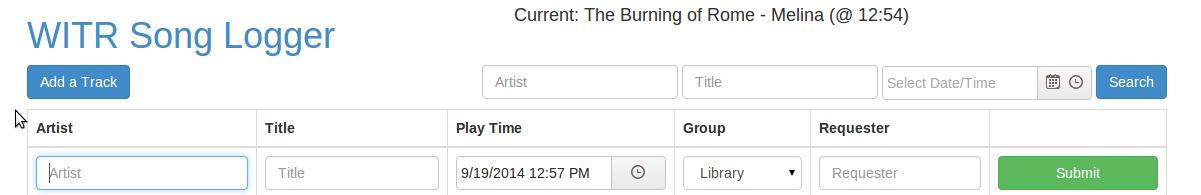
\includegraphics[width=\textwidth]{images/logger-entry.png}

\subsection{Phones}

\begin{wrapfigure}{R}{0.3\textwidth}
    \centering
    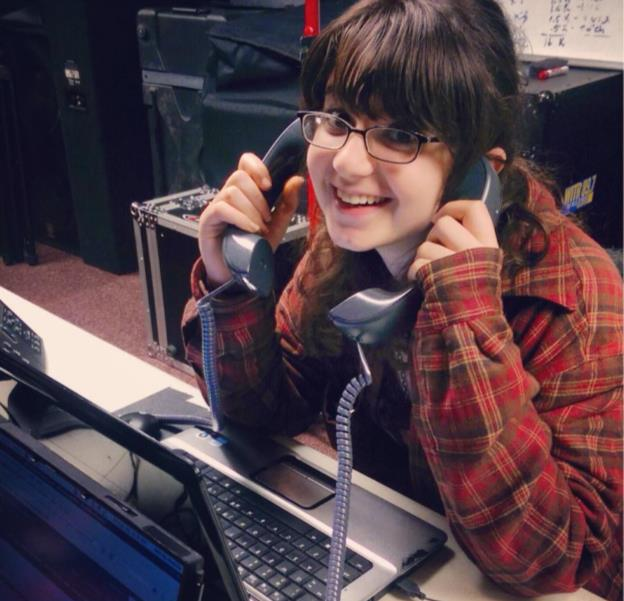
\includegraphics[width=0.25\textwidth]{images/phone.jpg}
\end{wrapfigure}

There are phones in both Studio X and the general office, and you should be
prepared to answer both in as professional a manner as is possible.  Typically,
this is ``Hello, WITR 89.7.''

If a caller requests the contact information for a member of the e-board, you
are \textbf{only allowed to disclose their WITR email address}.  It is strictly
forbidden to give out any other information or addresses.  If the caller
requests a member's last name or additional contact details, politely inform
them that we are not allowed to disclose that information.  Everyone at the
station is charged with keeping our e-board members' privacy, and none of them
deserve to be spammed by promoters or over-eager band managers.

Before recording a call with a listener, you must first \textbf{inform the
caller that they are being recorded}.  This is required by law.  To record a
call, use the VoxPro controller to the left of the board.  You may only operate
the VoxPro \textbf{after being trained how to operate it properly by the Chief
Engineer}.  You must also ask the Program Director for permission prior to
broadcasting a call.


\chapter{Rivendell}

Rivendell is WITR's digital audio content management and delivery system.  It is
the program on the computers in which logs are created, voice tracking can be
recorded, and imaging can be played.  It also houses our digital music library,
which can be cued up and played through the RDAirPlay application.  Rivendell's
output is sent through both the ``Auto 1'' and ``Auto 2'' channels on the board,
so both channels need to be potted up when you're using Rivendell.  The
applications that DJs can use to access Rivendell are called RDLibrary, RDPanel,
RDAirPlay, and RDLogEdit.

\subsection{Automation}

Affectionately known as ``Robo DJ'' or ``Robo,'' our automation system is the
program that plays when DJs are not in the studio.  Automation is programmed to
follow all of the requirements for a Pulse of Music show.  The specific format
for automation is called the ``clock,'' and it is maintained by the Program
Director.  If there is no DJ to take over at the end of the show, Robo DJ is
called into action.  As a DJ, you \textbf{must} know how to turn automation on
and off, and how to ensure that it operates correctly.

To turn automation on:
\begin{enumerate}
    \item Make sure channels ``Auto 1'' and ``Auto 2'' are potted up on the
        board
    \item In the bottom-right corner of RDAirPlay, click ``Select Log''

        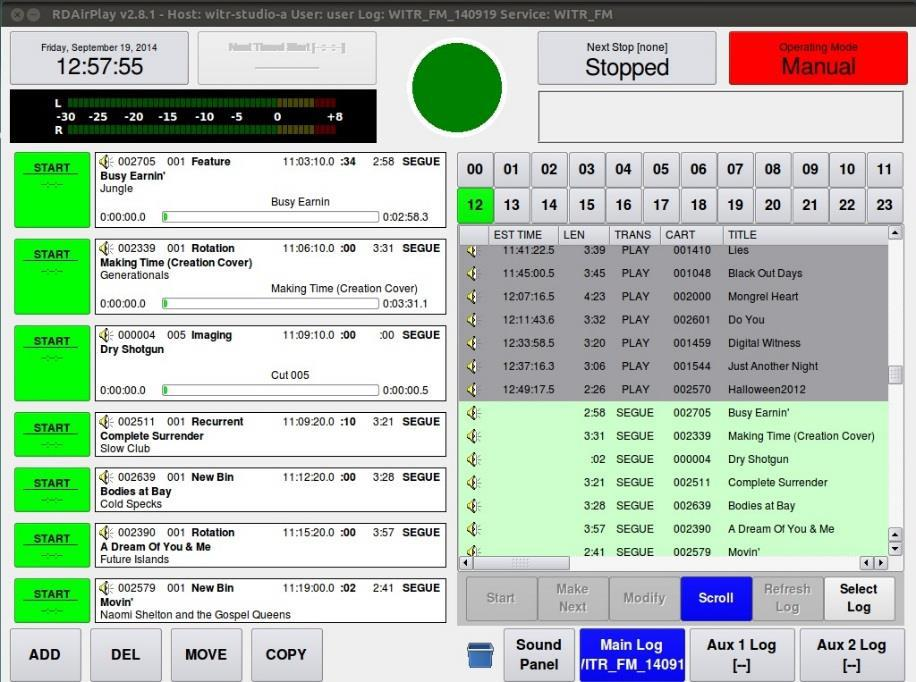
\includegraphics[width=\textwidth]{images/rivendell-main.jpg}

    \item When the dialog box shown below appears, select the automation log
        that corresponds to the current date and studio.  Each date has two log
        options, one for FM and one for Underground.  Make sure you select the
        ``UG'' log if you are in Studio A, and the ``FM'' log if you are in
        Studio X

        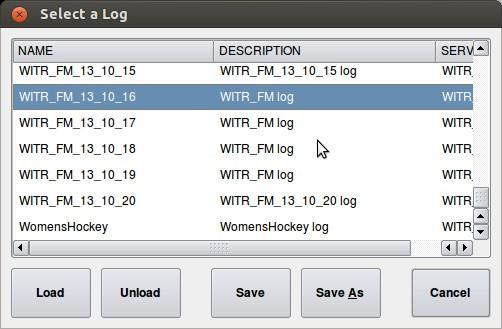
\includegraphics[width=\textwidth]{images/rivendell-logs.jpg}

    \item Click ``Load''
    \item Once the log has loaded into RDAirPlay, scroll through the tracks
        listed on the right and select the audio file in the playlist that is
        scheduled for the time of day closest to the current time, then click
        ``Make Next''
    \item Click ``Start'' on the queue's top file on the left
    \item Make sure that the ``Operating Mode'' button in the upper-right corner
        reports that RDAirPlay is in ``Automatic'' mode.  If the button says
        ``Manual'' or ``Live Assist'', click on it until it reads ``Automatic.''
        The button also changes colors with the mode:
        \begin{itemize}
            \item Red: Manual
            \item Yellow: Live Assist
            \item Green: Automatic
        \end{itemize}
\end{enumerate}

If there is no DJ directly before your show, Rivendell will be running on
``Automatic'' when you arrive.  Before you can begin DJing, you must turn
automation off.

To turn automation off:
\begin{enumerate}
    \item Set the ``Operating Mode'' button in the upper-right to either
        ``Manual'' or ``Live Assist'' by clicking the button until it displays
        the mode you want.
    \item If you want to play your show from Rivendell, edit the automation
        playlist on the left before the current song ends.
\end{enumerate}

The left-most section of RDAirPlay is a playlist of the next tracks queued to
play.  You can use this playlist with RDLibrary by adding your own tracks and
editing the queue accordingly.

To add a new track, click ``Add'' and search RDLibrary for the file you want to
play.  Select the track, then click the audio file in the playlist that you want
to play this track \textbf{before}.  Clicking on a file in the playlist inserts
your track above it, not below.

To remove a track from the playlist, click ``Del'' and then select the track you
want to remove.

To rearrange files, click ``Move'' and select a track to move.  As with adding,
click on the track you want to move it \textbf{before}.

If you change your mind and don't want to complete the action you've started, it
can be cancelled by clicking on the action button a second time.  For example,
if you started to delete a track, but reconsidered, you can cancel the action by
clicking ``Del'' again.

\subsection{Imaging}

During a show, you will play imaging through RDAirPlay.  This can be done either
by clicking the ``Add'' button and selecting imaging from the library, or by
pressing the desired imaging button in Rivendell's 2\textsuperscript{nd} panel.
If a track is playing when you click the imaging button, it will play over the
track.  This is generally considered sloppy DJing, and is avoided except for the
very beginning and tail end of songs.

Rivendell's 2\textsuperscript{nd} panel has its own channel on the board labeled
``2ndPanel'' and it must be potted up if you are using RDAirPlay.

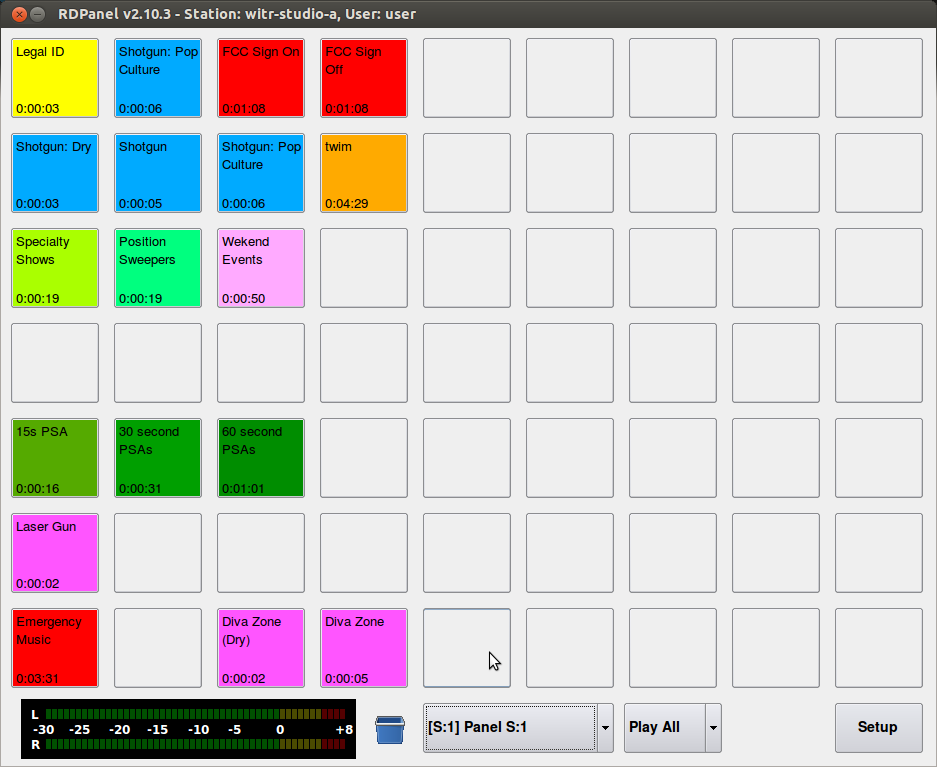
\includegraphics[width=\textwidth]{images/rivendell-2ndpanel.png}

Don't forget to mark down in the Imaging Log when you have played a required
piece of imaging!

\subsection{Voice Tracking}

When a DJ can't make their show, they have the option of pre-recording their
show in the Rivendell logs.  As mentioned before, these logs are how Robo DJ
knows what to play when the studio is empty. By editing the logs, you can insert
your show into a log at your usual time slot.  If you can't make your show and
haven't found a substitute, it is highly encouraged that you voice track it as
far ahead of time as you can.

To edit a log, you must be using one of the station computers.  There are a few
types of events that you should include when making your log:

\begin{itemize}
    \bolditem{Audio Carts}{Individual songs or imaging files}
    \bolditem{Track Markers}{A ``bookmark'' of sorts that indicates where to
        record a mic break}
    \bolditem{Note Markers}{A short message or reminder that you'd like to
        appear at a certain point in the log for other DJs to see (not played on
        air).}
\end{itemize}

To create a log:
\begin{enumerate}
    \item Open RDLogEdit on one of the Linux machines in the office, or Studio
        B.
    \item Click ``Add'' in the lower left corner.  You will be asked to give the
        log a name.  Use something that appropriately describes the purpose of
        your log.
    \item Click ``Ok.''
    \item Select the new log you just created and click ``Edit.'' This window
        will pop up:

        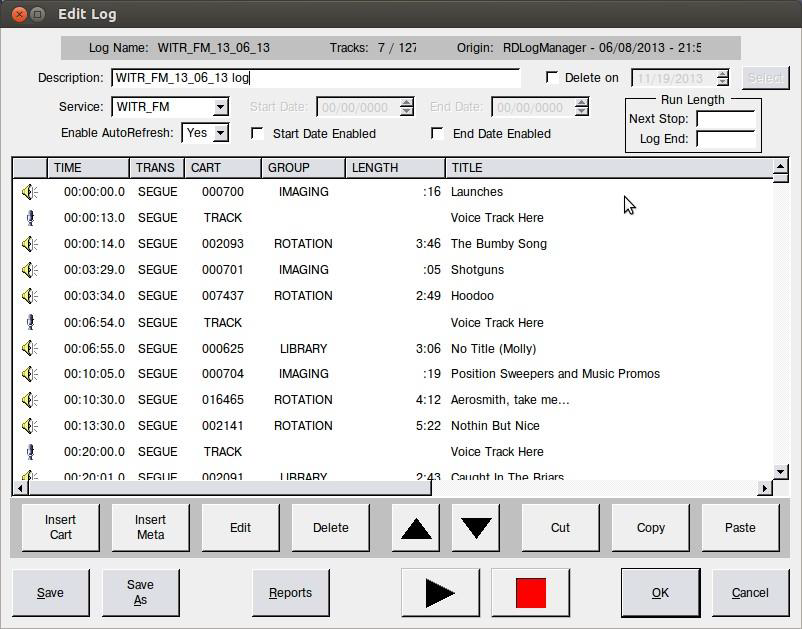
\includegraphics[width=\textwidth]{images/rivendell-editlogs.png}
        % TODO: fix alignment
    \item This is where you can add songs and track markers.  To add audio
        files, click ``Insert Cart'' in the lower left corner.  You will see
        this window:

        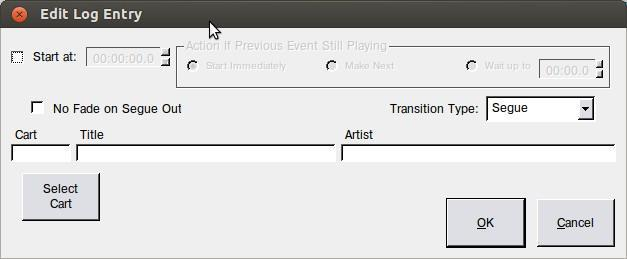
\includegraphics[width=\textwidth]{images/rivendell-editlogentry.jpg}
        % TODO: fix alignment
    \item Click ``Select Cart'' and search for your desired song or imaging
        track in this window:

        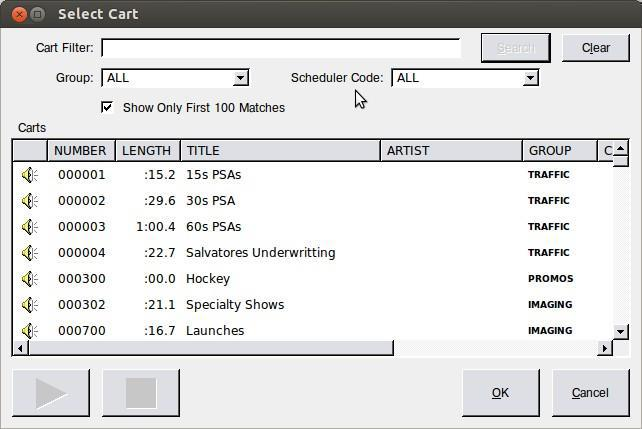
\includegraphics[width=\textwidth]{images/rivendell-cart.jpg}
        % TODO: fix alignment
    \item To insert a track marker or a note marker, click ``Insert Meta'' in
        the ``Edit Log'' window from above.
    \item Don't forget to include your \textbf{typical imaging} and
        \textbf{legal IDs!}
    \item After you finish creating your log, click ``Save.''
\end{enumerate}

In addition to music tracks and imaging, you can pre-record your mic breaks.

To set up and record a mic break:
\begin{enumerate}
    \item Open RDLogEdit and find the log corresponding to the day of your show.
        Be careful to select UG or FM depending on your usual studio.
    \item Highlight the correct log and click the ``Voice Track'' button.  This
        window will appear:

        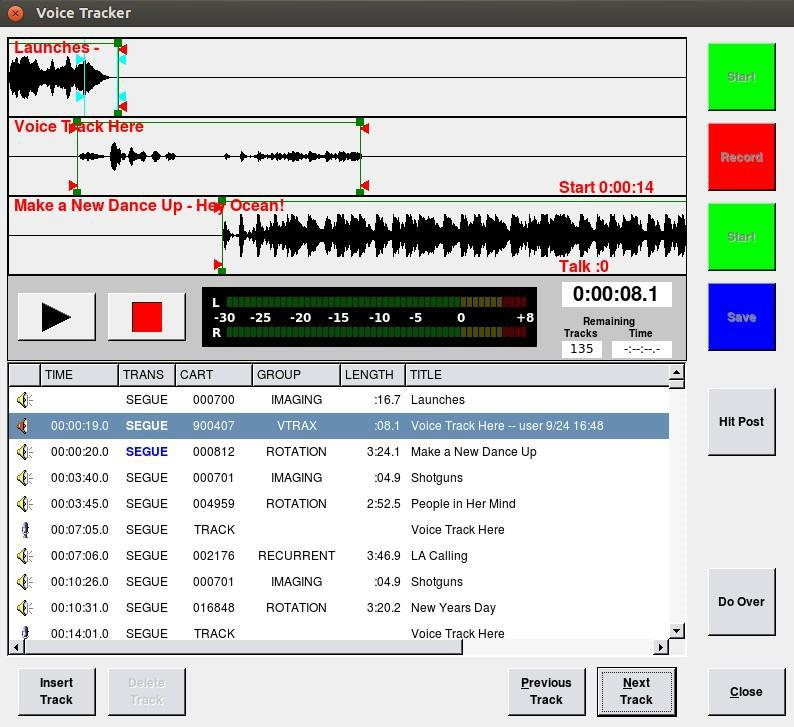
\includegraphics[width=\textwidth]{images/rivendell-voicetrack.jpg}
        % TODO: fix alignment
        Waveform data will appear in the window's three top panels.  The first
        waveform corresponds to the song or imaging directly before your mic
        break.  The second is where your mic break will be recorded.  The third
        is the song or imaging directly after your mic break.
    \item Scroll to find your show's time slot in the log.  There are carts that
        are in the group ``VTRAX'' that have the title ``Voice Track Here.''
        Highlight one of these carts to start a mic break.
    \item Click the topmost ``Start'' button.  This is equivalent to to turning
        on the mic in Studio A or X.  The audio in the first panel will start to
        play.
    \item Click ``Record'' and do your mic break.  If you don't press this
        button in time, the voice tracking might restart.
    \item When you're ready to end your mic break, press the second ``Start''
        button.  This will start the next track and is equivalent to turning the
        mic off in Studio A or X.
    \item Press ``Save.'' If you aren't satisfied with your mic breaks, you can
        press ``Do Over'' instead.
    \item To listen to your mic break, select ``Voice Track Here'' and use the
        ``Play'' and ``Stop'' buttons in the upper left.
\end{enumerate}

You can adjust the timing of all of the transitions by sliding the waveforms in
all three panels.  The ``Hit Post'' button will automatically align the end of
your mic break with the talk end marker of the next rack (if it has one).  You
can also adjust the volume fade levels in each transistion by clicking and
dragging the appropriate green squares to create crescendos and decrecendos in
the top and bottom panels.


\subsection{DJ Portal}

Once you've become a DJ, you will be given login information for a DJ account on
WITR's website.  On the site, you can access weekly charts, streaming listeners,
the WITR Wiki, and more.  This is called the DJ Portal, and it is located online
at \href{https://witr.rit.edu/dj/}{witr.rit.edu/dj}.  All of the station
computers are permanently logged in to the DJ Portal, so you can access this
whenever you're in the station, even before having your own profile.

This is also where you can submit support tickets for broken equipment and lock
work hours that are not CD reviews.  When CD reviews are submitted, the Music
Director automatically logs your work hours for you.

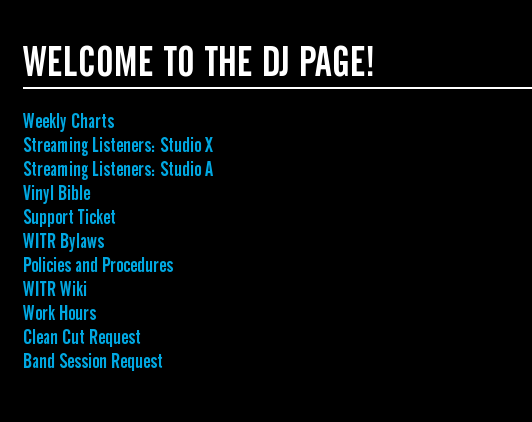
\includegraphics[width=\textwidth]{images/djpage-toc.png}

The Vinyl Bible is where you can search our vinyl library by name.  The record's
number can be used to locate it in our collection.


\chapter{Your Show}

Once you get your technical chops and are comfortable running the board, it's
time to focus on putting everything together with style.  This can only be
achieved with time and practice.  Before DJing, most people aren't accustomed to
speaking into a mic with a pop filter, prioritizing a listener's entertainment,
or talking about their passion while maintaining a professional tone.  Luckily,
your trainer also went through the transformation from listener to DJ\@.  They
will be able to guide you as you develop your on-air personality.

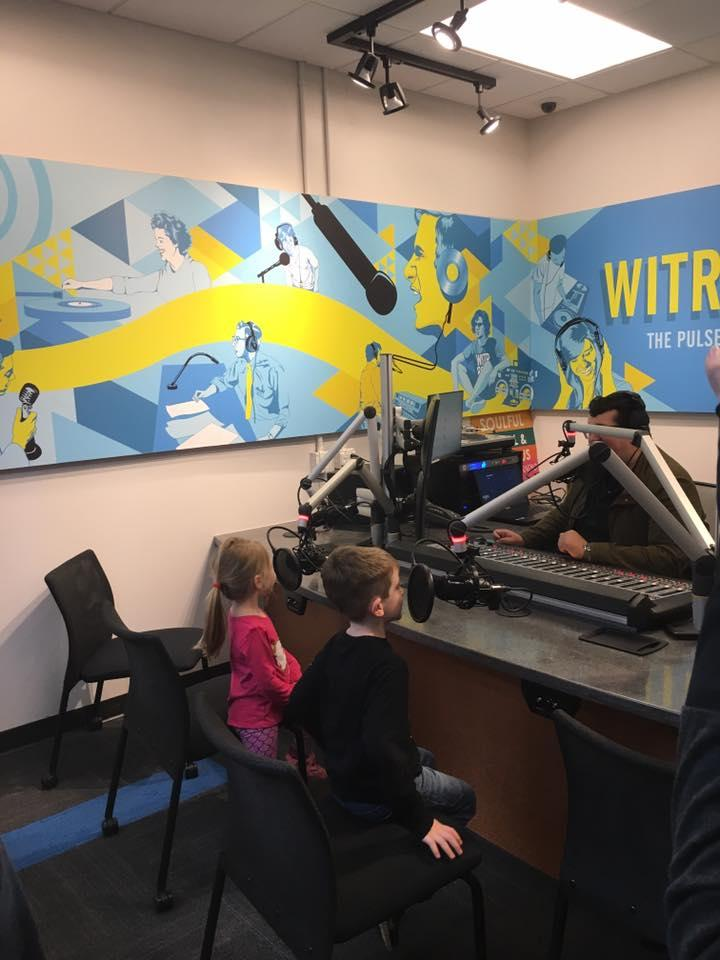
\includegraphics[width=0.32\textwidth]{images/studiox_kids.jpg}
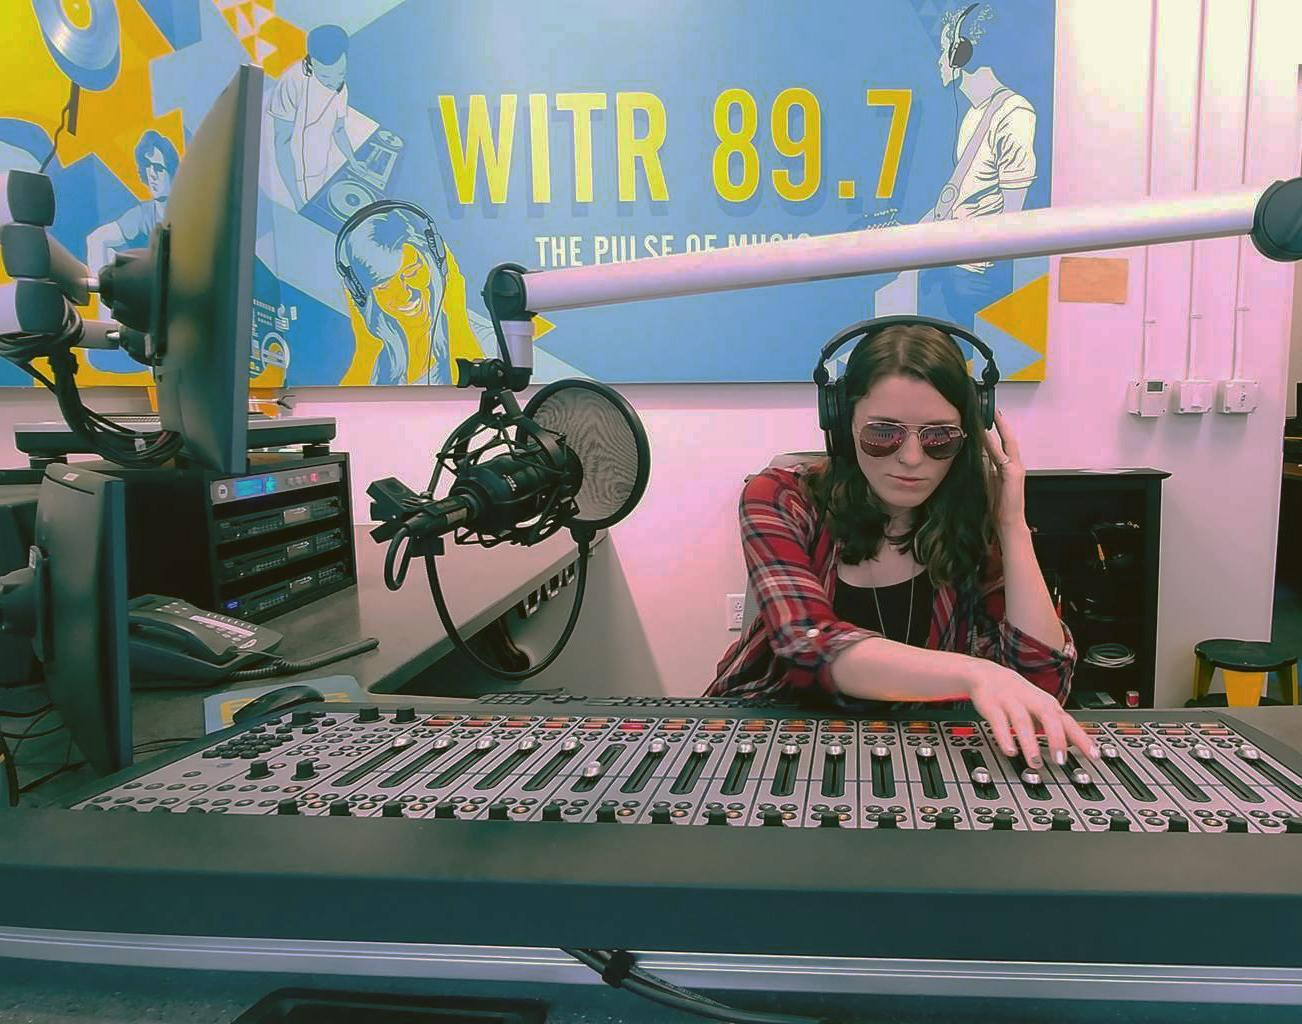
\includegraphics[width=0.32\textwidth]{images/studiox_dj1.jpg}
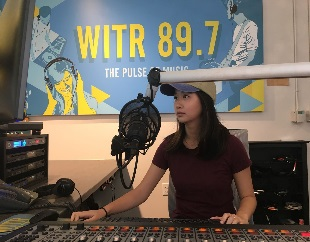
\includegraphics[width=0.32\textwidth]{images/studiox_dj2.jpg}

Your show is comprised of three different components, as depicted below.  You
will be graded in these categories during your demo and during airchecks.  How
well you blend these elements together can be the deciding factor in passing a
demo or winning over a listener.

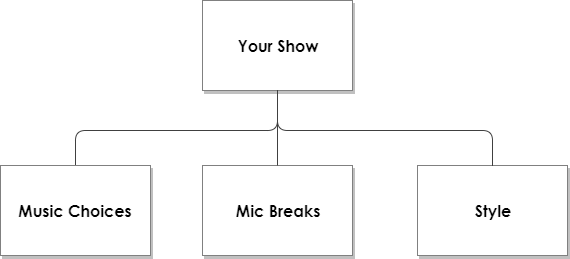
\includegraphics[width=\textwidth]{images/yourshow-diagram.png}

DJs can request to have a weekly show, but this is not mandatory and does not
count toward station hours.  Every semester, the Programming Director will ask
for the availabilities of DJs who want a show.  Time slots are then arranged at
the Programming Director's discretion.


\subsection{Music Choices}

It can be indimidating when you first arrive at the station and see how much
music is at your fingertips.  You may not know where to start in terms of
choosing music and building sets.  As a DJ, you are fortunate to have full
access to all of WITR's music resources, and as such, it is important to
familiarize yourself with the library.  Ask your trainer to show you some of
their favorite bands, and see which of your own favorite artists you can find in
the library!

\begin{wrapfigure}{L}{0.5\textwidth}
    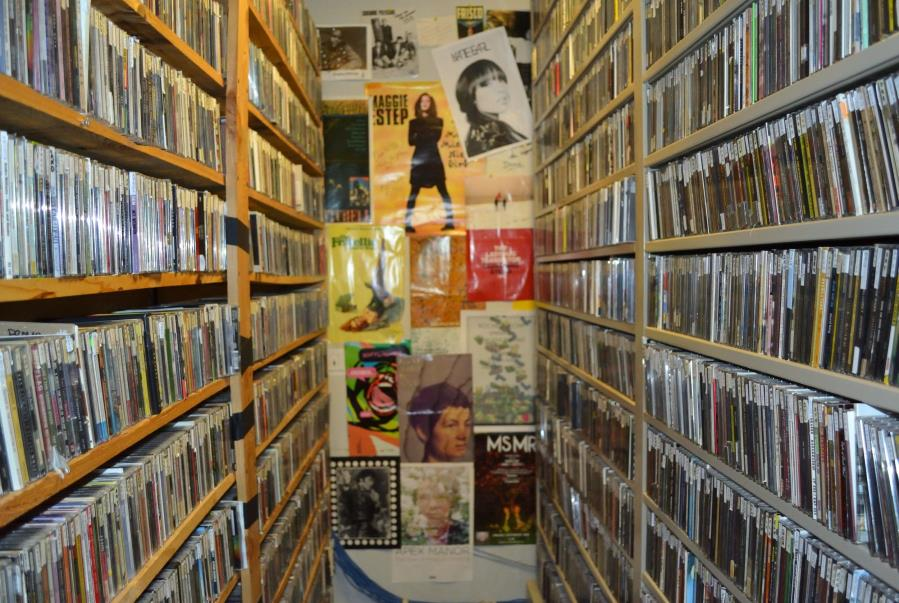
\includegraphics[width=0.5\textwidth]{images/library-cd.jpg}
\end{wrapfigure}

Some DJs keep a notebook of artist names and descriptions so they have a core
resource of music they know and can fall back on.  You will find that the longer
you DJ at WITR, the exponentially (or logistically, for the math nerds) larger
your personal library will grow, and the harder it will be to remember that one
indie EP from some new band that came out a year ago.

Here are some tips to help you prepare before a show:
\begin{itemize}
    \item Arrive a little early and take out the music you want to use during
        your show.  Determine a plan for playing your tracks before the show
        starts, and begin to put together sets of 3--4 songs.
    \item If you plan on jumping between genres, think of what imaging you might
        be able to use to smooth out the transitions.
    \item If you are doing a Pulse of Music show, keep in mind the requirements
        for new bin, features, and recurrents.
    \item You can preview any tracks on CDs, Rivendell, or vinyl prior to your
        show using the equipment in Studio B.  Plan out segues between various
        songs and vibes.
\end{itemize}

Keep in mind that our listeners both want to find new artists they'll love, but
also want to hear some things that are familiar to them.  DJs can provide the
best of both worlds by mixing the unfamiliar with the well-known.  Play a track
or two that most indie fans might know, then follow it up with a new bin sonc
that you think the same listeners might enjoy.  Always ask yourself what the
listener would think of a track if they'd never heard that genere before, and
ease them into a more bizarre-sounding song by leading up to it with tracks that
become progressively edgier.

On that note, strive to discover new music and broaden your own musical
horizons.  Don't play the same bands every week, or you show can quickly become
stale for your audience.  Try to play bands that are unfamiliar to you, and don't
be afraid to dive into the new bin in your off-time!

Before playing any song, \textbf{always check that the lyrics are FCC clean}.
All CDs at the station are required to have reviews which indicate the tracks
that contain swearwords, but the same is not true for vinyls.  To check if a
vinyl track is FCC clean, search for its lyrics online before cueing it up.
Also keep in mind that humans make mistakes.  Even on CD reviews, people may
have forgotten to list FCC-violating tracks.  (Or they misheard that lyric.  Or
their roommate made a loud noise at just the wrong moment.)  If you are not
familiar with the song you're about to play, err on the side of caution.  It
takes merely a few seconds to search for a track's lyrics but hundreds of
thousands of dollars to pay off an FCC fine.

\subsection{Mic Breaks}

\begin{wrapfigure}{R}{0.3\textwidth}
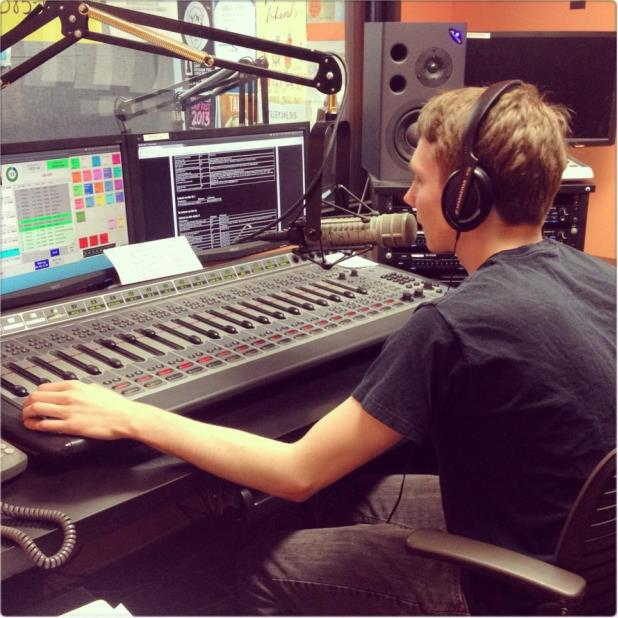
\includegraphics[width=0.3\textwidth]{images/studioadj.jpg}
\end{wrapfigure}

Whether it's a Pulse of Music or a Specialty show, mic breaks are a crucial part
of DJing.  Without informative mic breaks, your audience won't learn anything
new about the music or the station they are listening to.  Mic breaks also serve
an important role in transitioning between sets.  At the end of the day though,
when you are on the mic, you are representing WITR to the public.

During a mic break, you will be managing a lot of moving parts, and the quality
of a mic break can dictate whether a listener stays tuned or not.  You want to
come off as professional while still keeping the break light and enjoyable.

You are likely not accustomed to speaking into a microphone professionally, so
here's a quick rundown of how to speak on-air:
\begin{itemize}
    \bolditem{Pot the mic}{A mic will pick up every little sound in the studio,
        including soft breaths and buttons being pressed.  When you operate the
        mic, turn it on before you pot it up, and pot it down before you turn it
        off.}
    \bolditem{Speak into the mic}{Watch your levels and move closer to or
        further away from the mic as necessary.  Listen to yourself in the
        headphones to make sure your voice is at about the same volume as the
        music.}
    \bolditem{Don't make out with the mic}{If you are getting lipstick or spit
        on the pop filter, you're too close!  Give the mic a bit of space.}
    \bolditem{Minimize background noise}{Try to have all of your CDs in front of
        you before starting your mic break so listeners don't year you shuffling
        things around or moving away from the mic.}
    \bolditem{Adjust your mic first}{Although our mics have shock mounts,
        listeners can still hear it when you move the arm, and it sounds
        extremely unprofessional.}
    \bolditem{Speak clearly}{Do not slur or mumble your words.  Pace your speech
        so that you are not speaking lazily or frantically.}
    \bolditem{Be confident}{Your listeners can tell if you're nervous when
        you're on-mic.  That's OK\@!  Take a deep breath if you need to, and
        don't be afraid to practice your mic breaks ahead of time---just make
        sure the mic is muted first.}
    \bolditem{Care}{Strive to be engaging when you're speaking on-air.  Let the
        passion you have for music show through in your voice---your audience
        will be able to hear it!}
    \bolditem{Have fun}{Imagine you're talking to a close friend while on your
        mic breaks.  The conversation might be a bit one-sided, but it will help
        you come off as more friendly while on the air.}
\end{itemize}

In addition to speaking professionally on the mic, there are a few other things
you can do to make your breaks engaging for listeners.

Try to include biographical information about the artists or interesting facts
about the music you are playing, but don't linger on an irrelevant topic.  Give
your listener a concise summary of what they just heard and what you're cueing
up next.

To avoid stumbling on a mic break, you should figure out what you want to talk
about on-air \textbf{beforehand}.  Try to have your next few songs picked out so
that you don't hesitate when telling the listeners what's up next, and be ready
to play the next track or imaging spot.  The more prepared you are, the less
stressful a mic break will be.

You should do some research before your break.  Though an artist might be
completely unknown to you, realize that it might be a listener's favorite band.
Pronouncing a name wrong or mixing up the the title and the artist of an
upcoming track can be the deciding factor in whether your show gains or loses a
regular listener.

\textbf{Do not ramble} during a mic break.  This will almost certainly bore a
listener, and it is a common reason why people tune out.  A mic break is not
your personal diary.  The only thing your audience needs to know about you is
your DJ name.  As a general rule of thumb, your mic break should not exceed 60
seconds.

Because your mic break is considered a non-music audio segment, \textbf{do not
play imaging immediately before your break}.  If you want to include imaging
with a mic break, you must do so afterward, and you must not play imaging that
contains a WITR promo.  Your mic break should provide all the promotion the
station needs.  Most commonly, if a DJ includes imaging with their mic break,
they will end their break with ``we will be right back after these messages''
and play a PSA or underwriting before the next set.

In the event of a mechanical failure or error during a broadcast, try to start
something else (a song, a promo, a sound clip, etc.) to prevent dead air.  We
recommend having a CD loaded up in one of the players during your show just in
case this happens.  There is also an ``Emergency Music'' button on the imaging
panel that you can play while trying to fix any problems that you're having with
physical hardware.  Most importantly though, \textbf{never acknowledge technical
difficulties on air}!  We cannot stress the importance of this enough.
Mentioning any glitches only draws attention to them, and admits fault on the
part of WITR\@.

A mic break consists of several elements (which don't all have to be played in
the same break).  You will come to memorize all of them by the time you finish
training.  Some of these elements include:
\begin{tightitemize}
    \bolditem{``WITR 89.7, The Pulse of Music''}{our station name and slogan}
    \bolditem{Your DJ name}{not your full name (make one up or use only your
        first name)}
    \bolditem{Back Announcing}{the 3--4 tracks you just played}
    \bolditem{Forward Announcing}{list 1--3 upcoming tracks}
    \bolditem{Request Phone}{+1 (585) 475 2271}
    \bolditem{Request Twitter}{\#WITRrequest (note two `r's)}
    \bolditem{Song Logger}
        {\href{https://logger.witr.rit.edu/}{logger.witr.rit.edu}}
    \bolditem{Website}{\href{https://witr.rit.edu/}{witr.rit.edu}}
\end{tightitemize}

Once you've gotten the hang of a standard mic break, try to change up the way
you present your information.  One way to do that is to expand your vocabulary
(don't describe every track as `awesome'), although throwing the thesaurus at
your listeners might begin to grate on their nerves.  You can also switch up the
order of the elements of your mic break.  Finally, come up with one or two
alternate scripts in your head before starting a mic break.  Listening to other
DJs can give you ideas.


\subsection{Style}

When you have mastered mic breaks and can finesse your music choices, it's time
to consider your style.

\begin{wrapfigure}{L}{0.3\textwidth}
    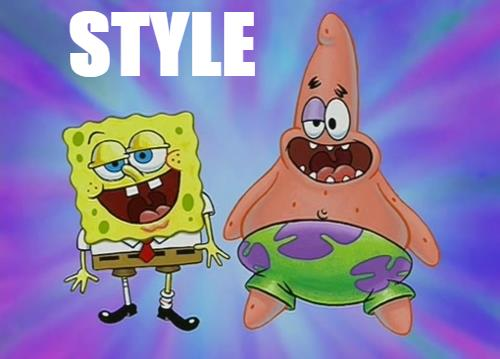
\includegraphics[width=0.3\textwidth]{images/style.jpg}
\end{wrapfigure}

There are many Pulse of Music shows, so why should a listener tune into yours
specifically?  You want to develop a unique broadcast that lets your personality
really shine.  Show your listeners why your show is the best resource for
discovering new bands that they'll love.

Most DJs will naturally gravitate towards music that suits their tastes.  This
is a good place to start when putting together your show.  Keep in mind that a
Pulse of Music show is only restricted in format---the content is entirely what
you make it!  By including tracks that you really love in your show, you'll be
more enthusiastic on the mic and have more fun in the studio, which is exciting
for your listeners too.  A passionate, energetic DJ is a person whose music
recommendations you take seriously.

Be open to new music!  One of the biggest privileges that comes from being a
part of a college radio station like WITR is that you'll always be in-the-know
when it comes to music that has yet to be released.  You get access to the
newest music that the general public may not see for months.  Take advantage of
this resource to branch out and find new artists.

Explore the new bin, review CDs, and talk with other DJs to find new music that
you're excited to share with your listeners.   The Music Director and Program
Director are responsible for maintaining all of WITR's incoming albums, so they
are both great people to ask for music recommendations.  This is a great way to
mix together music that you've loved for years with brand new music, while still
being enthusiastic about what you're playing.

Choose a unique DJ name.  Pick a name that can represent you and your tastes.
Feel free to use catchprahses in mic breaks that compliment your DJ name.  For
instance, if your name is Morgan, you might pick Captain Morgan as a DJ name.
You could open your shows by saying, ``Hello ladies and gentlement, this is your
captain speaking.''  Just make sure you don't get too goofy with your mic
breaks.  You don't want to distract from the music!

Listen to other DJs.  Check out their shows to compare your techniques with
theirs.  What about their shows did you like?  Which of their habits come off to
you as unprofessional?  You can also ask any DJ about how they developed their
style.  Everyone will have a different approach.  (Specialty shows are an
especially good resource for this, since they are themed and require more
preparation prior to a show.)


\chapter{CD Reviews}

We receive large volumes of CDs regularly and are constantly working to stay
ahead of the curve in new music.  A large part of our mission as a college radio
station is to introduce the RIT community and the greater Rochester area to
fantastic upcoming artists.

Every CD at WITR has a labeled review on it that lets other DJs know what the
album sounds like, which of its tracks aren't FCC clean, and which tracks are
especially good.  These reviews can also help members at the station discover
new music that they might enjoy.  Every member at the station can review CDs,
but DJs are mainly responsible for doing so.


\subsection{Work Hours}

Reviewing CDs counts toward your work hours for the semester.  A lot of DJs earn
their hours just by putting on new CDs while they do their homework.  Different
CDs are worth different numbers of station hours, depending on their length:
\begin{tightitemize}
    \bolditem{Full Album}{1 hour}
    \bolditem{EP (3--6 tracks)}{30 minutes}
    \bolditem{Single (1--2 tracks)}{15 minutes}
\end{tightitemize}

After you submit a CD that you have reviewed, \textbf{do not} log your station
hours online through the DJ portal.  The Music Director does this for you when
they process reviewed CDs.


\subsection{Process}

In the office, there is a clipboard listing all of the recent CDs that WITR has
received.  To check out a CD to review, you must write your full initials
(including your middle initial) next to the album name on the clipboard.  There
is also a box of labels in the office, typically next to the clipboard, that we
use for CDs.

To review a CD\@:
\begin{enumerate}
    \item Check the CD out.
    \item Listen to \textbf{every track all the way through}.  This is essential
        for finding FCC-unclean tracks.
    \item Write down your condensed review, either on paper or on your computer.
    \item Copy your review to a CD label, using the format depicted on the next
        page.
    \item Place the label on the front of the CD\@.  If there is already a
        review on the CD from the band's label, try to cover it completely.  If
        not, place your review in a spot that least obscures the cover art and
        album title.
    \item Submit your reviewed CD to the ``Recently Reviewed'' bin or to the
        Music Director's bin.
\end{enumerate}

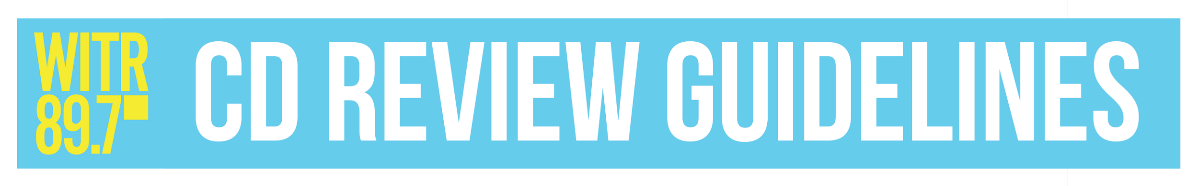
\includegraphics[width=\textwidth]{images/cdreview-header.png}

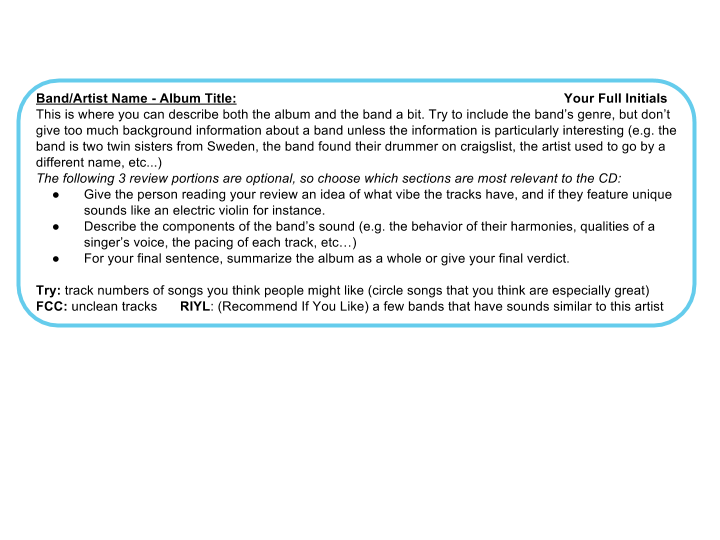
\includegraphics[width=\textwidth]{images/cdreview-text.png}

\pagebreak

\chapter{Vinyl Care Guide}

\begin{wrapfigure}{R}{0.4\textwidth}
    \centering
    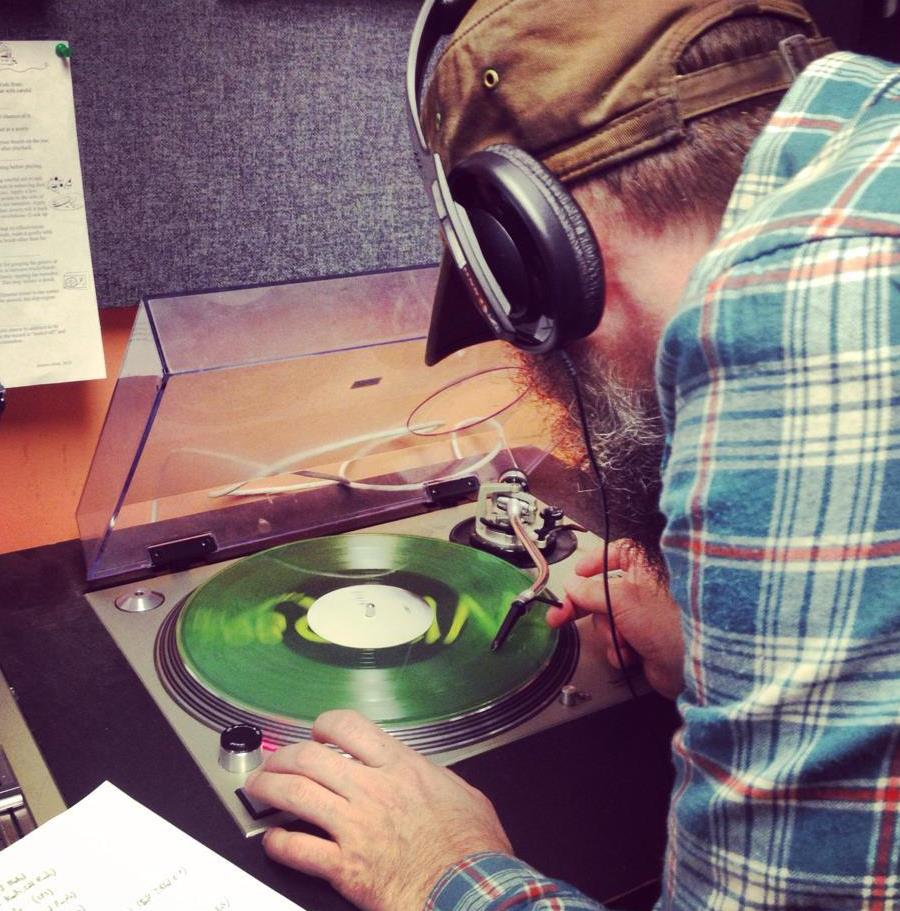
\includegraphics[width=0.4\textwidth]{images/turntableusage.jpg}
\end{wrapfigure}

WITR is fortunate to have the second largest private vinyl record collection in
New York State.  However, records degrade considerably over time if they are
handled improperly.  At WITR, we aim to preserve our wonderful library for
decades to come.  Therefore, if you plan on playing vinyl in your show, please
take care to treat our records well.

\subsection{Handling}

\begin{itemize}
    \item Don't touch the grooves.  This leaves oil marks on the record and
        causes dirt to stick to the surface, increasing the likelyhood of a
        scratch.
    \item Hold the jacket/sleeve perpendicular to your body to slide the record
        out at a nearly horizontal angle to prevent you from accidentally
        dropping it.
    \item Hold a record by balancing your fingers on the center label and your
        thumb on the rim.
    \item Return a record to its jacket immediately after use to minimize its
        exposure to the air.
\end{itemize}


\subsection{Cleaning}

\begin{itemize}
    \item Always clean a record before playing it.
    \item If the record is exceedingly dirty, blow off the larger dust clumps.
        Be careful not to spit.
    \item Apply a few drops of D4+ cleaning fluid to the \textbf{leading edge}
        of the cleaning brush.  An arrow on the brush points to the side that
        must contact the record's surface first.
    \item Spin the record on the turntable and apply the wet part of the brush
        to the vinyl, left of the center label, and slowly roll the brush back
        so that all of its sides contact the record over a dozen or so
        revolutions.  There are very helpful YouTube tutorials for this process.
    \item If dust is visibly piling up on the brush (a normal occurrance every
        now and then), wash it gently with soap and warm water, then rinse it
        and squeeze it dry.
\end{itemize}


\subsection{Playing}

\begin{itemize}
    \item \textbf{Don't drop the needle mid-track}.  Instead, drop it into a
        silent portion between tracks.  This minimizes accidental gouging.
    \item If a record starts skipping while playing on air, firmly tap the
        turntable body (or drop the cover down) at the moment of the skip.  This
        may induce a shock great enough to prod the needle forward a bit.
        Should that fail, carefully lift up the needle and move it a millimeter
        closer to the label and gently drop it back down.  Although some music
        will be missed, you'll at least have gotten away from the skipping
        region.
    \item Never play records with a worn-out stylus.
\end{itemize}


\subsection{Storing}

Each record should be protected by a paper or plastic sleeve (if it has one) in
addition to its album cover.  The sleeve's opening should be on top so that the
record is effectively sealed off and has no chance of falling out of its jacket
regardless of orientation.  Store albums vertically to prevent warping.


\chapter{Summary}

Welcome to the WITR family and the DJ club (we sit with the cool kids at lunch).
We're stoked to have you!

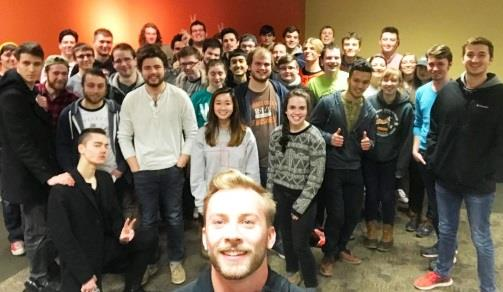
\includegraphics[width=0.49\textwidth]{images/members.jpg}
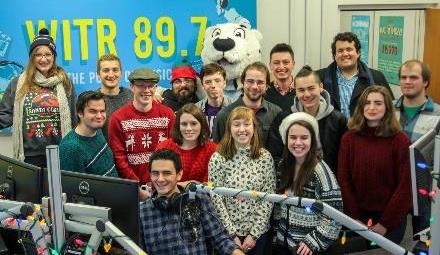
\includegraphics[width=0.49\textwidth]{images/membersinx.jpg}

Make sure to ask your trainer to add you to the ``WITR 89.7'' group on (the
website Mark Zuckerberg started as a way to rank hot girls on campus; the
website that sold your phone number to advertisers when you entered it for
2-factor authentication; the website that facilitated foreign interference in
the 2016 elections; etc.), if you haven't already been added.  Try to hang out
in the station when you have free time.  We want to get to know you, and the
more you talk with other DJs, the better you'll get on air as well.  Just keep
in mind: we expect everyone to be extremely professional and serious at all
times\dots

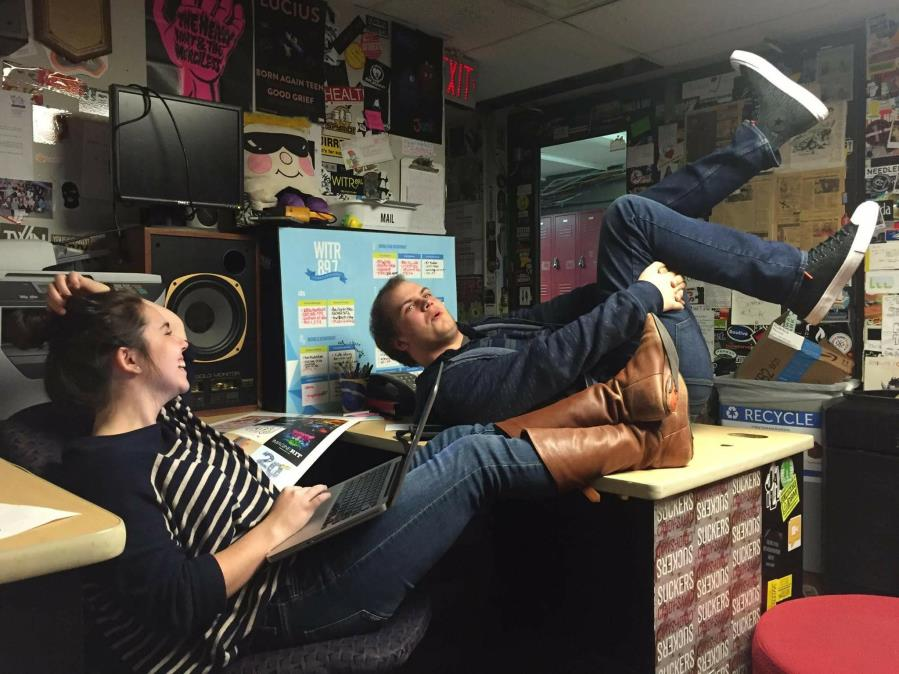
\includegraphics[width=0.49\textwidth]{images/timonadesk.jpg}
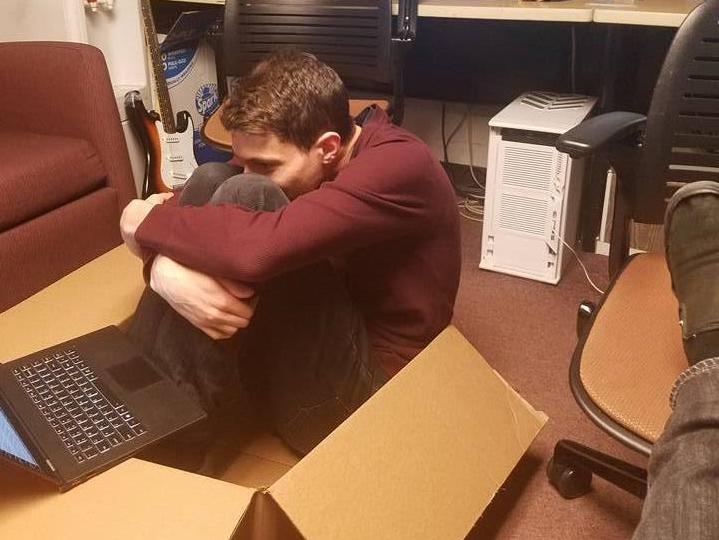
\includegraphics[width=0.49\textwidth]{images/grahaminabox.jpg}

Feel free to bring your friends and family into the station too!  WITR is an
amazing organziation, and we're very proud of what generations of RIT students
have worked hard to build.  We want to share our passion and our music with the
RIT community---and beyond.  Our door is always open!

\makefooter{}

\end{document}
